%!TEX root = ../thesis.tex
%*******************************************************************************
%*********************************** First Chapter *****************************
%*******************************************************************************

\chapter{Introduction \label{chap:1}}  %Title of the First Chapter

\ifpdf
    \graphicspath{{Chapter1/Figs/Raster/}{Chapter1/Figs/PDF/}{Chapter1/Figs/}{Chapter1/Figs/Vector/}}
\else
    \graphicspath{{Chapter1/Figs/Vector/}{Chapter1/Figs/}}
\fi


A new field of research related to both material science and condensed matter physics has been formed since the synthesis of graphene in 2004 \cite{Novoselov666,Novoselov26072005}. Graphene is a sheet of carbon atoms in a crystal form having a single atomic thickness. Given the thin plane-like structural nature of this type of material, the field is named two-dimensional (2D) material. The synthesis itself together with the phenomenal properties of graphene have led to a Nobel Prize in physics awarded to Andre Geim and Konstantin Novoselov in 2010 \cite{Geim2007}. Since then, the field is expanding with the involvement of researchers not only from the young community, but also from the experts who have been working on graphene-related materials like graphite, fullerenes and carbon nanotubes. As a result, research that focused on graphene and related topics are increasing with unprecedented speed, see \autoref{fig:grpapers} for the publications and the patents made in the last decade. While a part of the research has been to explore more on the properties of graphene itself and its applications, the other part has been concentrated on the discovery of new 2D materials. It has been evidenced from graphene, same materials having different dimensions can have different properties. For example, as compared to graphite, its monolayer graphene has superior mechanical properties and massless carriers to name a few. Therefore, many materials with hidden properties which will only manifest themselves in other dimensions are yet to be discovered. 


\begin{figure}[htbp!] 
\centering  
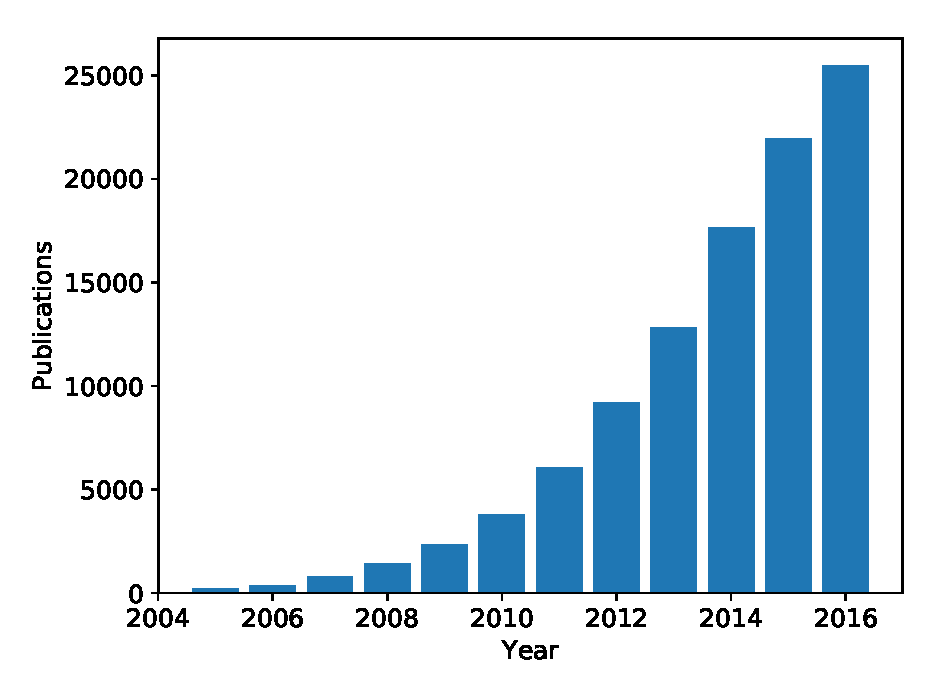
\includegraphics[width=0.8\textwidth]{graphene_papers.eps}
\caption[Graphene related publications and patents during the last decade]{Graphene related publications and patents during the last decade. Data source: ISI Web of Science and PATENTSCOPE. \protect\footnotemark }
\label{fig:grpapers}
\end{figure} 

On the other hand, with the advent of powerful supercomputer facilities, calculations that seems impossible to finish in a reasonable time now has been made possible. The accuracy of such calculations is the most crucial aspect of computational physics, especially when the results are utilized to predict real materials properties. To make the time spent on costly supercomputer valuable, researchers and programmers have been making important progress in order to make sure theories and its implementation are correct and the results they yield are within acceptable precision. Equipped with these tools, theoretical predictions have served well on discovering unexplored properties and applications of the materials. Moreover, detailed characterizations at atomic scale benefit the experimental results as well, or even to explain the unexpected outcomes.

\footnotetext{Publication and patent data are obtained by searching for "graphene" in the topic field of Web of Science and the title field of PATENTSCOPE, respectively.}

Considering all mentioned, it is a sound approach to apply state-of-the-art computational methods that are accompanied with high-performance supercomputer facilities to investigate the physical properties of novel 2D materials. This thesis was initiated to this end, and it is a summary of several works which have been accomplished during my Ph.D. study. The thesis is organized as follows: For the rest of this chapter, I will first introduce graphene and some other 2D materials that were discovered right after graphene, and, briefly, several well-known methods used to synthesis 2D materials. The following \autoref{chap:2} will present the computational methods, the theory and the implementations of them in available software packages. In \autoref{chap:3}, I will discuss several general properties of 2D materials. The next two chapters will be the main results of the thesis. Starting from specific properties targeting at specific novel 2D materials in \autoref{chap:4}, and followed by the modification of physical properties of 2D materials in \autoref{chap:5}. Overlaps of materials themselves and their properties are inevitable between sections, yet it will be minimized such that each section will have a unique topic. 



\section{Graphene}

Graphene is composed of carbon (C) atoms arranged on a honeycomb lattice in a single atomic layer. Graphite is made of van der Waals coupled graphene layers, see \autoref{fig:gra_grap}. These layers in graphite are stacked on top of another through weak physical bonds, whereas within each layer C atoms are held together by strong chemical bonds. As a result, it is possible to just isolate a single layer from graphite without damaging the layer itself. 

\begin{figure}[htbp] 
\centering  
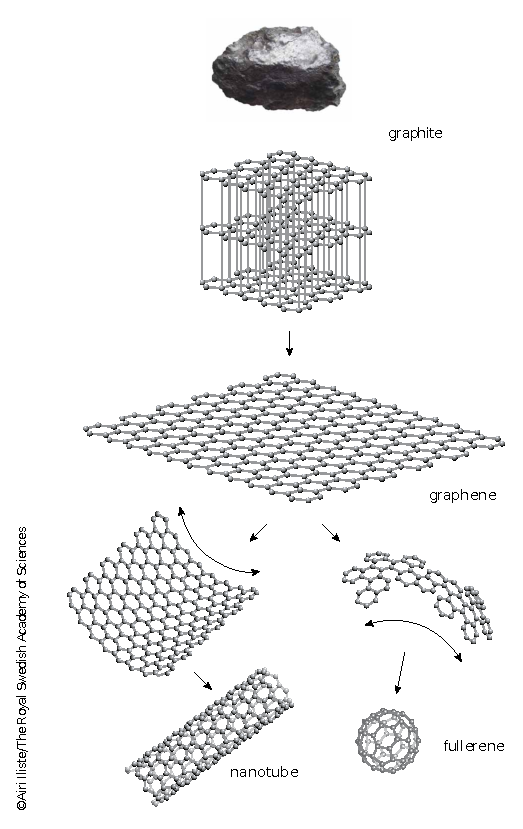
\includegraphics[width=0.7\textwidth]{gra_grap.eps}
\caption[Relation of graphite, graphene, fullerene and nanotube]{Relation of graphite, graphene, fullerene and nanotube. Image source: the Nobel prize in physics 2010 \cite{gra_grap}}  
\label{fig:gra_grap}
\end{figure} 


\subsection{History}

The story of graphene can be traced back to the discovery of graphite around 1564 in England\cite{petroski1990pencil}. Ever since, people have been using graphite, the tip of a pencil, for writing and drawing. The black trace left behind by a pencil is actually stacks of graphite and graphene, and by chance, even a single layer of graphene can present.  Apart from being a part of a pencil, graphite certainly has been holding a more important position in technology and industry due to its rich chemistry, low friction, high electrical and thermal conductivity etc. On the other hand, the synthesis of a single layer graphene seems to be discouraged by both experimental and theoretical limitation. On the experimental side, there have been attempts\cite{Krishnan1997,Ohashi1997,Dresselhaus2002,Shioyama2001} to isolate graphene from graphite or even grow it on a substrate. However, they failed mostly due to the poor control of the number of layers and the difficulty to identify graphene itself.  Addition to these experimental difficulties, theoretically, it was believed that strictly 2D materials should not exist because of a divergence in the thermal fluctuation in 2D materials that will make them unstable \cite{Peierls1935,Landau1937,Mermin1968}. Nevertheless, graphene was still considered as a theoretical model. For example, \citet{Wallace1947} was the first one to study the band structure of graphene \cite{CastroNeto2009}, and found some of the interesting properties, like a semimetallic band structure. 

Although not in the form of graphene, the single atomic layer of graphite has been already seen and studied in the other forms, e.g. fullerenes and nanotubes, see \autoref{fig:gra_grap}. These materials usually contain certain types of characteristic defects that make it different from graphene.  Fullerene has a quasi-spherical hollow ball shape. It is composed of both six- and five-folded C rings, where the latter give positive curvature and made the closed surface possible. The resulting shape resembles a football\cite{Kroto1985,Lamb1990}. The Nobel prize in chemistry of 1996 was award to Harold W. Kroto, Robert F. Curl and Richard E. Smalley for their discovery of fullerene. Another important type of carbon allotrope is carbon nanotubes\cite{Iijima1993}, and it was discovered by using the arc-discharge method\cite{Lamb1990} which was originally designed to produce a large quantity of fullerenes. Despite sharing similar production method, carbon nanotubes are actually more close to graphene than fullerene due to the absence of pentagonal C rings in the former two. A carbon nanotube can be constructed by rolling up a graphene sheet into a hollow tube as its name suggest. Carbon nanotubes are typically observed to have micrometer in lengths and nanometer in diameter and having either metallic or semiconducting nature depending on the way they are rolled up. They possess superior mechanical properties. For example, individual nanotube has a Young's modulus of 0.64 TPa and it is 56 times stronger than steel wire\cite{Baughman787}.

In 2004, the situation has changed completely for graphene with the successful isolation of a single layer of graphene from graphite by A. K. Geim and K. S. Novoselov at Manchester University using a simple micromechanical cleavage method. Except for a more sophisticated experimental control, the key ingredient for their success, as compared to the previous failures\cite{Krishnan1997,Ohashi1997}, is that the Si wafer underneath the graphene made it easier to identify graphene\cite{Geim2007}. The synthesis of graphene itself already is a ground-breaking achievement, however, what excited the researcher the most is the extraordinary properties that graphene has. In the following section, I will summarize some of them to illustrate this point.

\subsection{Physical properties}

As mentioned previously, graphene is a single atomic layer of graphite. It has an interesting structure with high symmetry which many of its properties are attributed to. Each C atom has three neighbors to which it is chemically bonded. Because of this, C atoms are arranged in a honeycomb lattice\footnote{Honeycomb lattice is not a Bravais lattice.}, or a hexagonal Bravais lattice with two atoms per site, see (a) in \autoref{fig:gra_band}. Graphene has a uniform bond length of 1.42\AA~ and uniform bond angles of 120\textdegree. The band structure which characterizes the electronic properties of graphene has been calculated by P. R. Wallace in 1947 \cite{Wallace1947}. He discovered that graphene is a semimetal with conduction band minimum (CBM) and valence band maximum (VBM) touch each other at the K and K' points in the first Brillouin zone as shown in (b) and (c) in \autoref{fig:gra_band}. The energy-momentum dispersion is approximately linear in the vicinity of the K and K' points. Due to this, the electron and the hole in those states behave differently as they do in a quadratic band. This has several consequences. First of all, considering the linear energy momentum relation, particles can be regarded as zero-mass Dirac particles and they are governed by relativistic Dirac equation\cite{Novoselov2005}, and they travel at a constant speed of \si{10^6m/s}. Hence, the K and K' points are referred as Dirac points, their vicinities are called Dirac cones. Secondly, the carrier concentration can be tuned continuously from electron to hole with a perpendicular electric field\cite{Geim2007}. Thirdly, the carrier in graphene can tunnel through a finite height potential without reflection if it normally incident to the barrier — Klein tunnelling\cite{Katsnelson2006}. Fourthly, under a particular magnetic field, a zero energy Landau level appears, and the large energy interval between the zero and the first level made it possible to observe the quantum Hall effect at room temperature \cite{Novoselov1379}, etc.

\begin{figure}[htbp!] 
\centering  
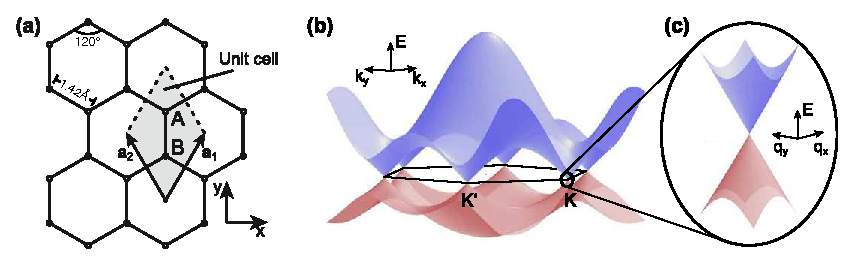
\includegraphics[width=\textwidth]{gra_lat_band.eps}
\caption[Graphene lattice and band structure.]{(a) Graphene honeycomb lattice composed of A and B hexagonal Bravais sublattices. (b) Band structure of graphene where CBM and VBM touch each other only at the K and K' points. (c) Approximately linear dispersion around the K and K' points. Image source: Ref. \cite{Guttinger2012} }  
\label{fig:gra_band}
\end{figure} 

Graphene delivers more than just interesting electronic properties. For example, evidencing the extraordinary mechanical properties, graphene has a Young modulus of 1Tpa and intrinsic strength of 130 Gpa\cite{Lee385}. This makes graphene the strongest material ever measured. More than 300 times stronger than steel and four times harder than diamond. High carrier mobility is another exciting feature that has more applicative importance in electronic devices. Free standing graphene without substrate attached has been reported to has carrier mobility of 230,000 \si{cm^2/Vs} at low temperature\cite{Bolotin2008a} and 120,000 \si{cm^2/Vs} at 240 Kelvin, the latter value is higher than that of any known semiconductor\cite{Bolotin2008b}. In addition, the thermal conductivity of graphene can reach up to 5000 \si{W/mK} at room temperature, which is 20 times higher than that of copper\cite{Alexander2008}. Despite these, having a zero band gap strongly suppressed the potential of graphene in digital logic gates applications. This is because the current controlled by the gate bias can not be turned off completely in graphene. To overcome this, efforts to opening a band gap in graphene have been made through substrate induction\cite{Ci2010,zhou2007}, bilayer graphene\cite{mccann2006,castro2007}, chemical adsorption\cite{Elias2009,Jeon2011}, chemical doping\cite{zhou2008} and quantum confinements\cite{Nakada1996,Barone2006}.  Doping and adsorption usually come with a price of reducing mobility by introducing scattering centres, chemically pure. In contrast, bilayer graphene and nanoribbon are thought to be promising approaches to open a band gap as well as, to a great extent, preserve graphene's superior intrinsic properties.

\section{Post-graphene materials and their general properties}

Excitements of the exploration of graphene have driven the force to discover more types of 2D materials. Researchers have taken different approaches to this end. On the one hand, aiming to open a band gap in graphene, chemical functionalizations on graphene have been carried out with chemical adsorption of hydrogen, fluorine and oxygen, and resulting in graphane, fluorographene and graphene oxide, respectively. On the other hand, inspired by graphite's layer structure, other layered materials are brought to the attention and efforts were undertaken to isolate a single layer of it. In this section, I will introduce some of these early post-graphene materials and their physical properties in general.

\subsection{Functionalized graphene}

\subsubsection{Graphane}

The full hydrogenation of graphene gives a 2-D hydrocarbon called graphane. It can be synthesized either by reduction of graphite and then hydrogenation of the left product (graphene, carbon nanotubes or graphite oxide) with liquid-based\cite{Yang2012} or gas-based\cite{Burgess2011} environments. I can be also grown by chemical vapour deposition\cite{wang2010}. 

Graphane is not flat as graphene. In fact, the bonding character changed from sp$^2$ hybridization to sp$^3$, which results into a buckled structure, see \autoref{fig:gra_h}. Neighbouring H atoms located at the different sides of the graphane plane. Among different phases of graphane, the chair structure was found to be the ground state. Others phases are metastable like boat, twist-boat and twist-boat-chair\cite{Samarakoon2009}. The C-C bond length in the chair structure is 1.52 \AA~and thus larger than that in graphene. Graphane is a semiconductor with 3.5 eV band gap in the chair form. The band gap was reported to scale almost linearly with the hydrogen coverage\cite{Ilyin2011}. The 2D Young's modulus of graphane is estimated 245 \si{N/m}\cite{Munoz2010} and thus smaller than 340 \si{N/m} of graphene. The incomplete coverage of H atoms on graphene gives hydrogenated graphene. It has a ferromagnetic magnetic state\cite{Zhou2009}, tunable band gap\cite{Shkrebtii2011} and reversible hydrogenation\cite{Elias2009}. 

\begin{figure}[htbp!] 
\centering  
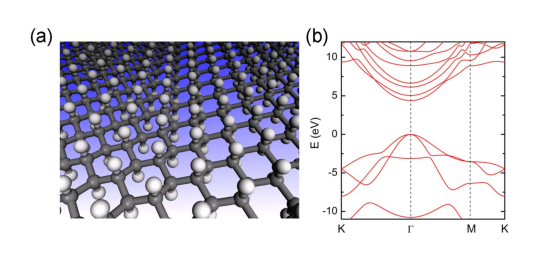
\includegraphics[width=1\textwidth]{graphane.eps}
\caption[Atomic and electronic structure of graphane]{(a)The chair structure of graphane. The white balls are the H atoms and the grey ones are the C atoms. Image source: Ref. \cite{Sofo2007} (b) Band structure of chair graphane. Image source: Ref. \cite{leenaerts2010}}  
\label{fig:gra_h}
\end{figure} 

\subsubsection{Fluorographene}

Stronger binding between an external atom and a C atom can be realized using fluorine atom for adsorption. A fully fluorinated graphene is called fluorographene, and it can be regarded as a single layer of graphite fluoride. In fact, sonochemical exfoliation of fluorographene from graphite fluoride is one of the ways to synthesis it, see \autoref{fig:gra_f}\cite{Zhu2013}. Fluorographene has a similar structure as graphane due to the same sp$^3$ hybridization, and it also has different isomers where again the chair type is the ground state configuration\cite{samarakoon2011}. The unit cell of fluorographene is around 1\% larger than that of graphene\cite{nair2010}. The formation energy of fluorographene is about 0.5 eV per fluorine atom lower than that of graphane per hydrogen atom\cite{Jeon2011}. The band gap of fluorographene is larger than 3 eV from optical measurement\cite{nair2010,Jeon2011}, and the band structure is similar to that of graphane with a band gap at the $\Gamma$ k-point. The 2D Young's modulus of fluorographene is 100 \si{N/m} and the intrinsic strength is about 15 \si{N/m}. Both are more than two times less than those for graphene due to the weaker sp$3$ bonds in fluorographene\cite{nair2010}.

\begin{figure}[htbp!] 
\centering  
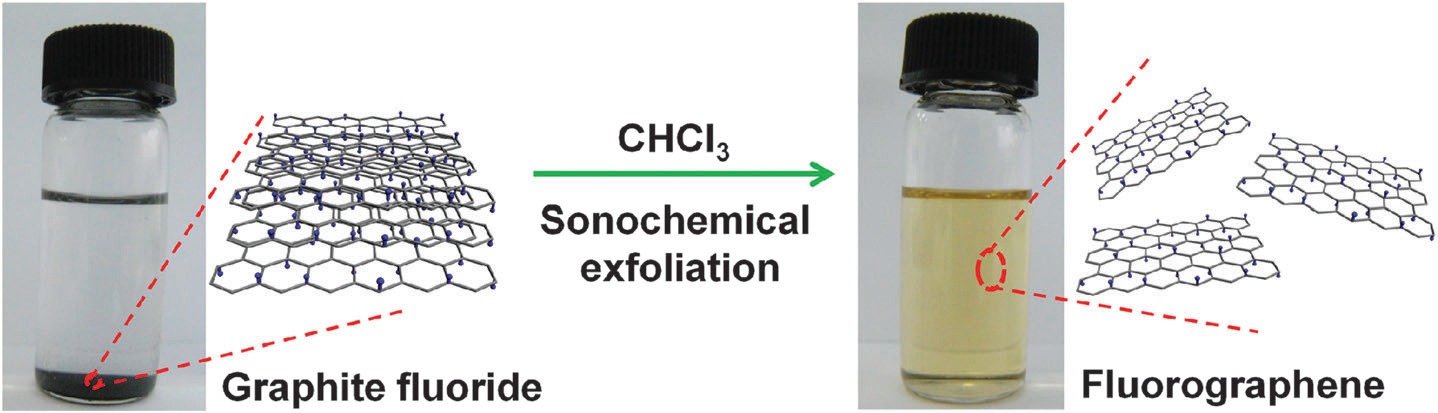
\includegraphics[width=1\textwidth]{fluorographene.png}
\caption[Graphite fluoride to fluorographene]{Graphite fluoride to fluorographene. Image source: Ref. \cite{Zhu2013}}  
\label{fig:gra_f}
\end{figure} 

\subsection{Group IV 2D materials}

Analogues to graphene, 2D materials made of only single elements from the other members of group IV elements have been also proposed and synthesized. These are silicene, germanene, stanene which are made of silicon (Si), germanium (Ge) and tin (Sn) atoms, respectively. They generally suffer from less stability as compared to graphene. The free standing form of these materials are difficult to make, instead, they usually need ordered substrates to support them. Therefore, the measurements that have done on these type of systems can not exclusively speak for the target material, the influence of the substrate is not negligible\cite{Lin2013}. This will, in turn, hinder the accurate determination of their properties. Despite of these experimental difficulties, theoretical studies have more freedom to investigate their physical properties. One of the most important differences of these materials as compared to graphene is their not-flat buckled structure, see \autoref{fig:silicene}. The buckling parameters $\delta$ is defined as the interlayer distance of layers at different 2D atomic planes. According to calculations, $\delta$ is 0.45\AA~for silicene, 0.69\AA~for germanene and 0.85 \AA~for stanene\cite{matthes2013}. This change corresponds to a more sp$^3$-like character in the orbitals, and it increases with the atomic radius. 

\begin{figure}[htbp!] 
\centering  
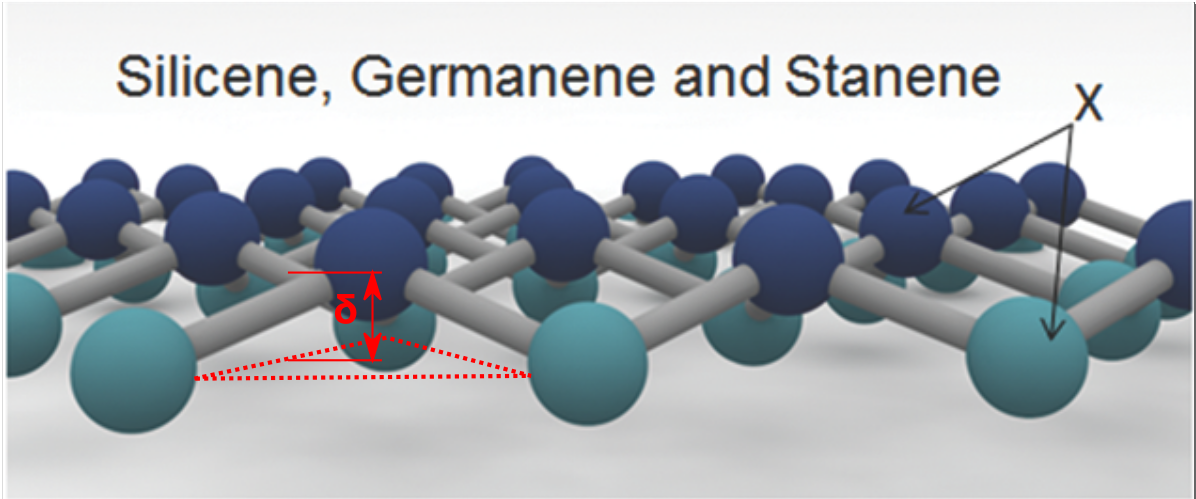
\includegraphics[width=0.9\textwidth]{silicene_structure.png}
\caption[Group IV 2D materials]{Buckled hexagonal crystal structures of group IV 2D materials (X = Si, Ge, and Sn). Different colors represent different 2D atomic planes and their distance is the buckling parameter $\delta$. Image is adapted from Ref. \cite{Balendhran2015}.}  
\label{fig:silicene}
\end{figure} 


Although having a buckled structure, these materials also possess Dirac points with linear energy momentum dispersion around them\cite{Garcia2011}.  However, as stated before, the substrate that supports these materials will induce symmetry breaking which leads to the loss of the Dirac character of the electrons/holes\cite{Lin2013} in these materials. Moreover, spin-orbit coupling (SOC) in these materials are predicted to be larger than that in graphene due to larger atomic weights. With the inclusion of SOC, this corresponds to 1.9 meV band gap in silicene and 101 meV of that in stanene\cite{matthes2013}. The mechanical stiffness and strength are lowered as compared to graphene and has a reducing trend with increasing atomic number in this group. This is partially due to the fact that the bond angle deformation in the buckled structure is less costly in energy than bond stretching in a flat structure\cite{Manjanath2014}. For example, silicene has a 2D Young's modulus around 62 \si{N/m}, that is four times smaller than graphene. Another important difference of these materials from graphene regards the realization of a monolayer. The lack of layered bulk counterpart of these materials made the mechanical exfoliation inapplicable, which is believed to produce the highest quality sample. Therefore, methods used in this case are either bottom-up decomposition techniques onto highly ordered substrates\cite{vogt2012,Linfei2014}, or top-down methods like chemical exfoliation to isolate grown target monolayer from substrate\cite{lin2012,kaloni2013}.


\subsection{2D from layered materials}

The layered structure of graphite contributes the most to the isolation of graphene. If the interlayer bonding were not the weak vdW interaction but rather a covalent type, even the concept of layers can not stand let alone to break the bonds only in one direction and keep others in the other two directions. Therefore, a reasonable way to explore other 2D materials is through other layered materials, e.g. hexagonal boron nitrides, transition metal dichalcogenides. In this section, I will discuss the general physical properties of these two materials as examples for 2D materials from layered materials.

\subsubsection{Boron Nitride}

Among the multiple structural phases of Boron Nitride, the layered hexagonal phase (h-BN) is the most stable one, see \autoref{fig:BN} for the structure. A single layer extracted from h-BN gives 2D h-BN. Because of its structural similarity to graphene and its wide band gap it is often referred as white graphene\cite{alem2009atomically}. 2D h-BN has a band gap of 6.1 eV according to calculations. An intuitive tight binding analysis reveals the band gap, in the case of 2D h-BN, to be proportional to the difference of p$_z$ orbitals from B and N atoms. For silicene and graphene, this difference is zero thus so is the band gap. Moreover, as a result of different electronegativity, i.e. 2.0 for B and 3.0 for N, ionic character develops which further enlarges the band gap\cite{zhuang2012}. Several interesting features of this material are reported: strong mechanical stiffness and strength close to graphene\cite{Bosak2006}, a good thermal conductivity of 100-270 \si{\watt\per\meter\per\kelvin} for few-layer h-BN\cite{Jo2013} as an electrical insulator, a high oxidation resistance up to 700 \si{\celsius} in contrast to 400\si{\celsius} for graphene\cite{li2016atomically}, etc. Benefiting from its compatible bond length, i.e. 1.446 \AA, with graphene (1.42), it is a perfect partner for graphene to form heterostructure electronic devices  and to serve as a dielectric substrate\cite{Lee2013}. Resulting system gives a larger mobility for graphene as compared to SiO$_2$ substrate\cite{dean2010boron} for instance. 


\begin{figure}[htbp!] 
\centering  
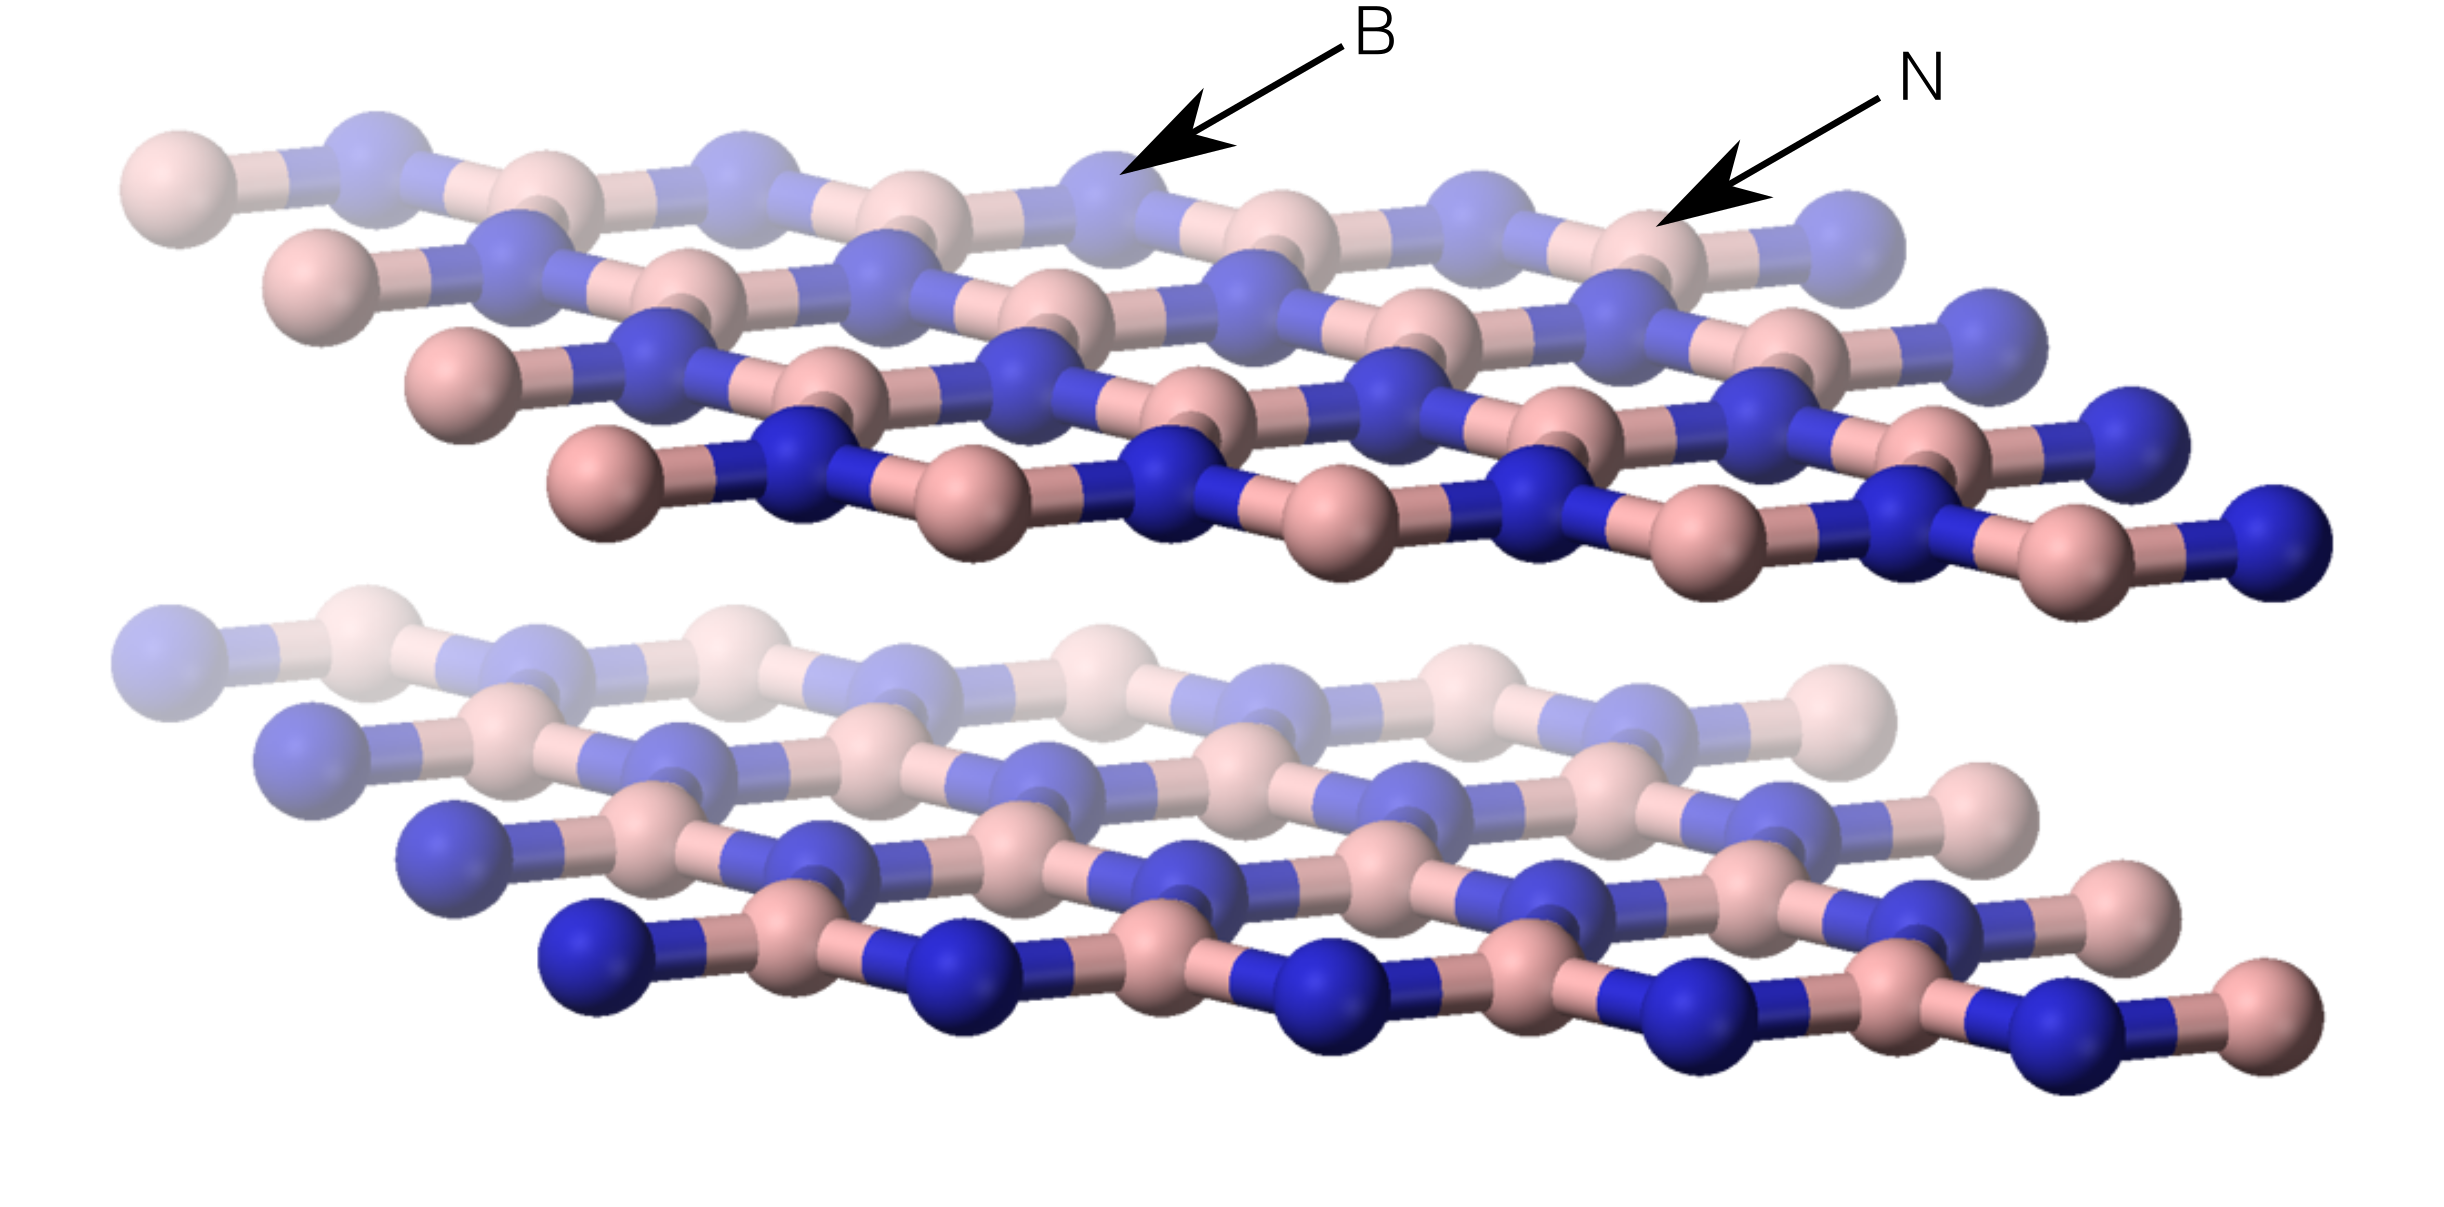
\includegraphics[width=0.9\textwidth]{BN.png}
\caption[Layered hexagonal structures of h-BN]{Layered hexagonal crystal structures of h-BN. Image is adapted from Ref. \cite{Benjah2007}.}  
\label{fig:BN}
\end{figure} 


\subsubsection{Transition Metal Dichalcogenides}

\begin{figure}[htbp!] 
\centering  
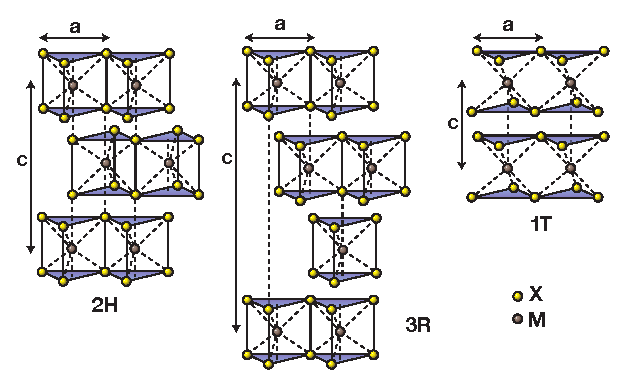
\includegraphics[width=0.9\textwidth]{tmds.eps}
\caption[Layered structures of TMDs]{Layered structures of TMDs. 2H: two layers per unit cell with hexagonal symmetry; 3R: three layers per unit cell with rhombohedral symmetry; 1T: one layer per unit cell with tetragonal symmetry. $a$ is the in-plane lattice constant with a range from 3.1 to 3.7 \AA~in TMDs. $c$ is the vertical lattice constant. The interlayer distance has a typical length of 6.5 \AA. Image source: Ref. \cite{Wang2012}}  
\label{fig:tmds}
\end{figure} 

Transition metal dichalcogenides (TMDs) have a general formula of MX$_2$, where M stands for the group 4-7 elements in the transition metal series in the periodic table, and X is the group VI element. This is another type of layered materials, and the single layer of some of them have been experimentally realized.  These materials typically exist in three different structural phases as shown in \autoref{fig:tmds}, which at monolayer level can be either H or T phase. One of the most important differences in these two phases is the lack of inversion symmetry in H phase in contrast to the T phase. Therefore, spin orbit coupling (SOC) becomes more important in H and induces spin-splitting. For instance, 456 meV electron spin states splitting in WSe$_2$\cite{Zhu2011giant} has been reported. Note that, inversion symmetry is recovered in the layered bulk form hence suppresses SOC. Another important consequence of reducing dimensionality is the indirect-to-direct band gap transition from layered TMDs to its 2D counterpart, see for example \autoref{fig:tmds_bands}. 2D-TMDs have a broad range of potential applications. Electrocatalysis\cite{kim2013enhanced,huang2014synthesis} benefits from adequate active sites, electronic devices\cite{RadisavljevicB2011,sun2014fabrication} benefit from typical band gap of 1-2 eV, Li or Na batteries\cite{chang2011cysteine,chen2013situ} benefit from high surface-to-volume ratio and short diffusion path, photocatalysis benefits from high stability under extreme light intensity\cite{Li2013,Parzinger2015}, and biomedicine benefits from enhancement of the physiological stability and biocompatibility of polymers on 2D-TMDs\cite{Cheng2014,Yin2014}. 



\begin{figure}[htbp!] 
\centering  
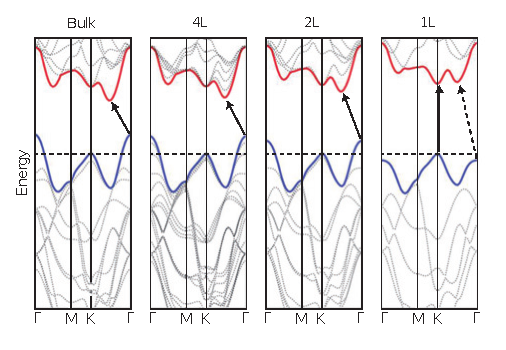
\includegraphics[width=0.9\textwidth]{tmds_bands.eps}
\caption[Band structure evolution of MoS$_2$ from bulk to single layer]{Band structure evolution of MoS$_2$ from bulk to single layer. Image source: Ref. \cite{Chhowalla2013}}  
\label{fig:tmds_bands}
\end{figure} 


\section{1D from 2D: nanotubes and nanoribbons}

The reduction of materials dimensions did not stop at the 2D level. Further lowering it will result in 1D nanotubes or nanoribbons. A nanoribbon is a strip of a 2D sheet with nanoscale width and microscale length and it is still flat. Whereas nanotubes are the rolling up of nanoribbons into a tube structure. Each nanotube, as well as each nanoribbon but with different definition, is associated with a chiral vector that uniquely defines its structure parameters except for the length which is considered to be infinite in theory. In \autoref{fig:chiral}, $\vec{a_1} $ and $\vec{a_2}$ are the unit lattice vectors in graphene. Chiral vector, $\vec{C}$, is the superposition of these two unit vectors with indices pair ($n$,$m$). Zigzag edge always has a ($n$,0) form and ($n$,$n$) is always an armchair edge. Everything else is called chiral type edge.  This finite-length chiral vector also defines the radius of the tube. Nanoribbons, on the other hand, have these three types of edges as well, however, in this case, edges have infinite length.

Having confinements from other directions, physical properties of these systems are expected to be different than that for their higher dimension counterparts. For example, graphene nanoribbons have a finite band gap in contrast to the zero band gap of graphene\cite{Wang2008}. Moreover, control of this confinement will give tunable physical properties. For example, the band gap in graphene nanoribbon has a overall inverse relation with the width of the nanoribbon\cite{Han2007}. The zigzag edges in graphene nanoribbon form spin-polarized magnetic states and give ferromagnetic ordering along the edge and anti-ferromagnetic ordering across the edges\cite{Son2006}. For nanotubes, those having the same edges belong to the same class of chirality and have the same electronic structure. For instance, armchair carbon nanotubes are metallic, other types are semiconducting. But small radius tubes can be exceptional due to the large curvature\cite{Bandaru2007}.  The strong mechanical strength and high thermal conductivity of a graphene nanoribbons and nanotubes are similar to those in graphene.

\begin{figure}[htbp!] 
\centering  
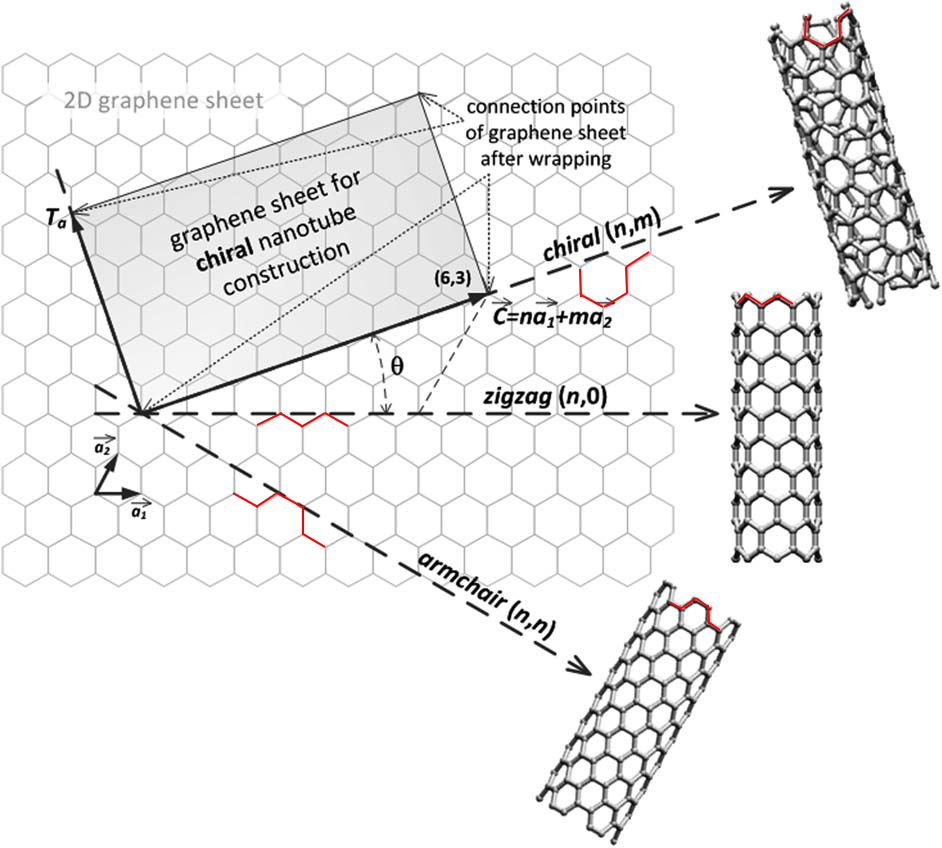
\includegraphics[width=\textwidth]{chiral_vector.png}
\caption[Chiral vector and different type of nanotubes as obtained by rolling them up in different directions]{Chiral vector and different types of nanotubes as obtained by rolling them up in different directions. Image is adapted from Ref. \cite{Prasek2011}.}  
\label{fig:chiral}
\end{figure} 

\section{Synthesis methods}

In this last section, I will briefly discuss some of the well-known synthesis methods for 2D materials. In \autoref{fig:syn}, an overview of graphene production methods is displayed. 

\begin{figure}[htbp!] 
\centering  
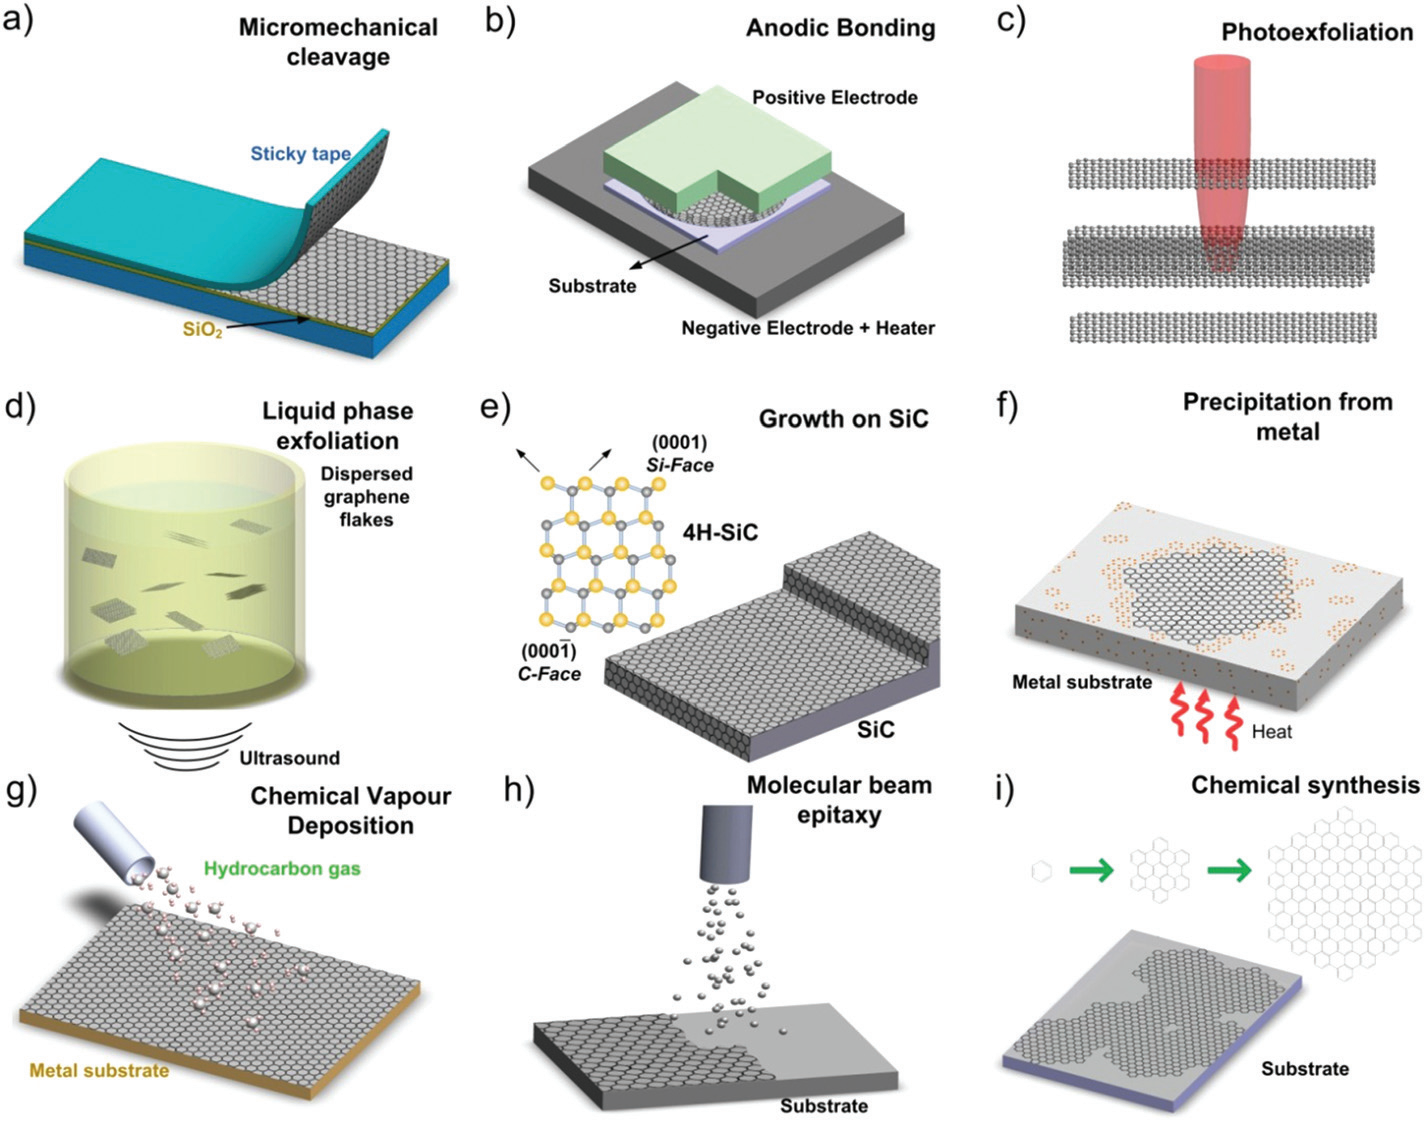
\includegraphics[width=0.9\textwidth]{synthesis.png}
\caption[Graphene production setups]{Graphene production setups. Image source: Ref. \cite{Ferrari2015}}  
\label{fig:syn}
\end{figure} 
\subsubsection{Micromechanical cleavage}

Micromechanical cleavage is also known as mechanical exfoliation, which was the method used to the first successful isolation of graphene in 2004 using an adhesive tape\cite{Novoselov26072005}. It involves separating layers in layered materials by mechanical, electrostatic, or electromagnetic forces. This method gives high-quality product and is suitable for laboratory-scale sample that is ideal for fundamental studies. Large scale productions are impractical through this method.  Room temperature mobility was measured up to 20,000 cm$^2$V$^{-1}$s$^{-1}$\cite{Ni2010} on graphene prepared with this method.

\subsubsection{Liquid phase exfoliation}

Liquid phase exfoliation is the extraction of layers in a proper solvent using ultrasounds. The cavitation-induced bubbles collapse around the graphite will generate a compressive stress wave. As a primary result, this will cause a reflective tensile wave whose strength is proportional to the number of such bubbles. Intensive tensile stress is enough to break graphite into graphite flakes. Additionally, as a secondary effect, shear effect can be developed from the unbalanced lateral stress and separates two adjacent layers. Liquid phase exfoliation is a promising method to synthesis cheap and scalable samples. 

\subsubsection{Growth on SiC}

The growth of graphene on SiC involves Sic sample annealing at high temperature ( > 1400\si{\celsius}) in a vacuum or under an atmospheric pressure. The sublimation of silicon atoms leaves behind carbon atoms on the surface which will rearrange to form a graphitic layer\cite{Mishra2016}, see \autoref{fig:sic}. Apart from having high reproducibility and the ability to grow homogeneous large-area sample, this method has the advantage that graphene is available on a semiconducting substrate already for a layered electronic device integration. 

\begin{figure}[htbp!] 
\centering  
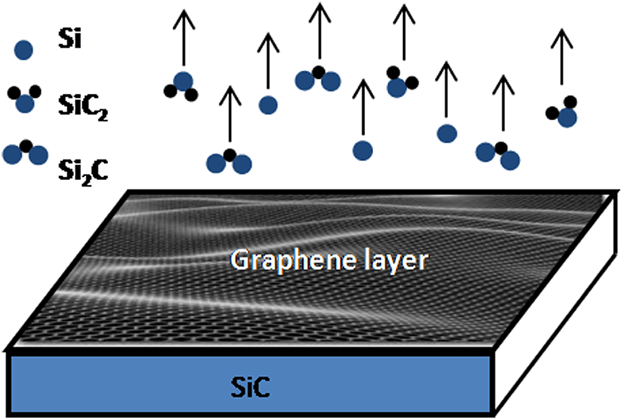
\includegraphics[width=0.6\textwidth]{gr-sic.png}
\caption[The growth of graphene on SiC wafer]{The growth of graphene on SiC wafer. Image source: Ref. \cite{Mishra2016}}  
\label{fig:sic}
\end{figure} 

\subsubsection{Chemical vapor deposition}

Chemical vapor deposition (CVD) is a popular method to grow amorphous or crystalline thin film from solid, gaseous or liquid precursors. It is a direct deposition of vaporized desired material onto a particular substrate. Various CVD methods exist depending on their operating pressure, types of vaporization and whether it is plasma-assisted or not etc. Graphene grown on transition metals usually is of high quality. Carbon atoms from organic sources in the gas phase are deposited on a metal (Ni, Ru, Ir etc.) and convert to graphene at high temperature. Then, for the characterization, graphene is transferred to a proper substrate. Typical mobility of such type of sample is around 1000-25000 cm$^2$V$^{-1}$s$^{-1}$\cite{Petrone2012}. A 30-inch graphene film has been produced from roll-to-roll production through CVD methods by \citet{Bae2010}, see \autoref{fig:30gr}. The product was measured to be a better electrode than commercially available indium tin oxides.

\begin{figure}[htbp!] 
\centering  
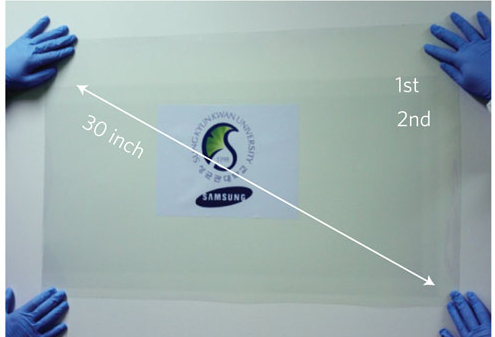
\includegraphics[width=0.7\textwidth]{30-inches-gr.jpg}
\caption[An ultra-large-area graphene film]{An ultra-large-area graphene film. Image source: Ref. \cite{Bae2010}}  
\label{fig:30gr}
\end{figure} 

